%%%%%%
%
%  @@@@@@@ lrlab report template @@@@@@
%  Use this template only for lab-internal reporting events.
%
%  DO NOT USE THIS FOR YOUR ACADEMIC ORAL PRESENTATIONS 
%  including intermediate and final master's presentations
%
%%%%%%
%% Set the compiler to LaTeX on Overleaf
%%%%%%
%% Comment out one of the two \documentclass lines
%%%%%%
%% normal documcent view (portrait)
\documentclass[]{lrlabreport}
%% use `slide' option for screen (landscape) presentation view
%\documentclass[slide]{lrlabreport}

\usepackage{lrlabreport} % lrlabreport.sty
\bibinput{sample} % required by usebib.sty called in lrlabreport.sty

%%%%%%%%%%%%%%%%%%%%%%%%%%%%%%%%%%%%%%%%%%%%%%%%%%%%%%%%%%%%%%%%%%%%%%%

% define here your commands as you want
% E.g., \newcommand{\eg}{\textit{e.g.,}}

%%%%%%%%%%%%%%%%%%%%%%%%%%%%%%%%%%%%%%%
%%% title page content
%%%%%%%%%%%%%%%%%%%%%%%%%%%%%%%%%%%%%%%

\title{\color{blue} Research theme, or 1-liner summary of this report}
%% never use contentless/helpless title such as Seminar, Summary, Report, etc.

\author{Student's name in both Latin alphabet and 漢字 (if you have)}
\date{Report/Presentation Date}

\begin{document}

\maketitle
\begin{abstract}
\noindent\begin{itemize}
    \item Show the summary of this report in an itemized presentation
    \item 1. what you did
    \item 2. what you obtained
    \item 3. what you will do
\end{itemize}
\end{abstract}
\thispagestyle{empty}

%%%%%%%%%%%%%%%%%%%%%%%%%%%%%%%%%%%%%%%
%%% body content
%%%%%%%%%%%%%%%%%%%%%%%%%%%%%%%%%%%%%%%

\section{Overview/研究概要}

\I This section is mandatory
\I Show 1-page\tinyfn{In case of screen view. Otherwise, not applicable} summary of your research 
\I Explain the objective, the core idea/approach, and expected contributions


\section{Recap/前回(まで)のまとめ}

\I This section is mandatory unless this is the first report
\I Show 1-page summary of your previous report(s)


\section{Current report content/今回の報告内容}

\I You can freely organize the remaining part

\I Use \verb|\section| to start a section\tinyfn{You should not try to match each section to 1 page. 
\textbf{This format is not intended to prepare slides. Essentially this is a paper-like document template.} Therefore, when you have a presentation with a material using this template, use the continuous-scroll view (e.g., a web page) rather than the page-by-page view.} as many as you like

\I Use `screen view' when you report in-person, i.e., w/ the `slide' option of \verb|\documentclass|

\I You should write this document in `document view' at first, i.e., w/o the `slide' option


\I Use \verb|\I| for itemizing a description easily like this
%\I If you like, you can also use the \verb|itemize| environment

\I Use \verb|\paper| to cite a paper like \paper{devlin-etal-2019-bert} with its title in a footnote

\subsection{Note (this is a subsection)}
{\small \redcolor You can also use normal text descriptions for detailed information. Just like this paragraph you are currently reading. However, such descriptions should be skipped in the oral presentation.}

\subsection{Figure example/図の例}

\begin{figure}[H] % forcing `here'
    \centering
    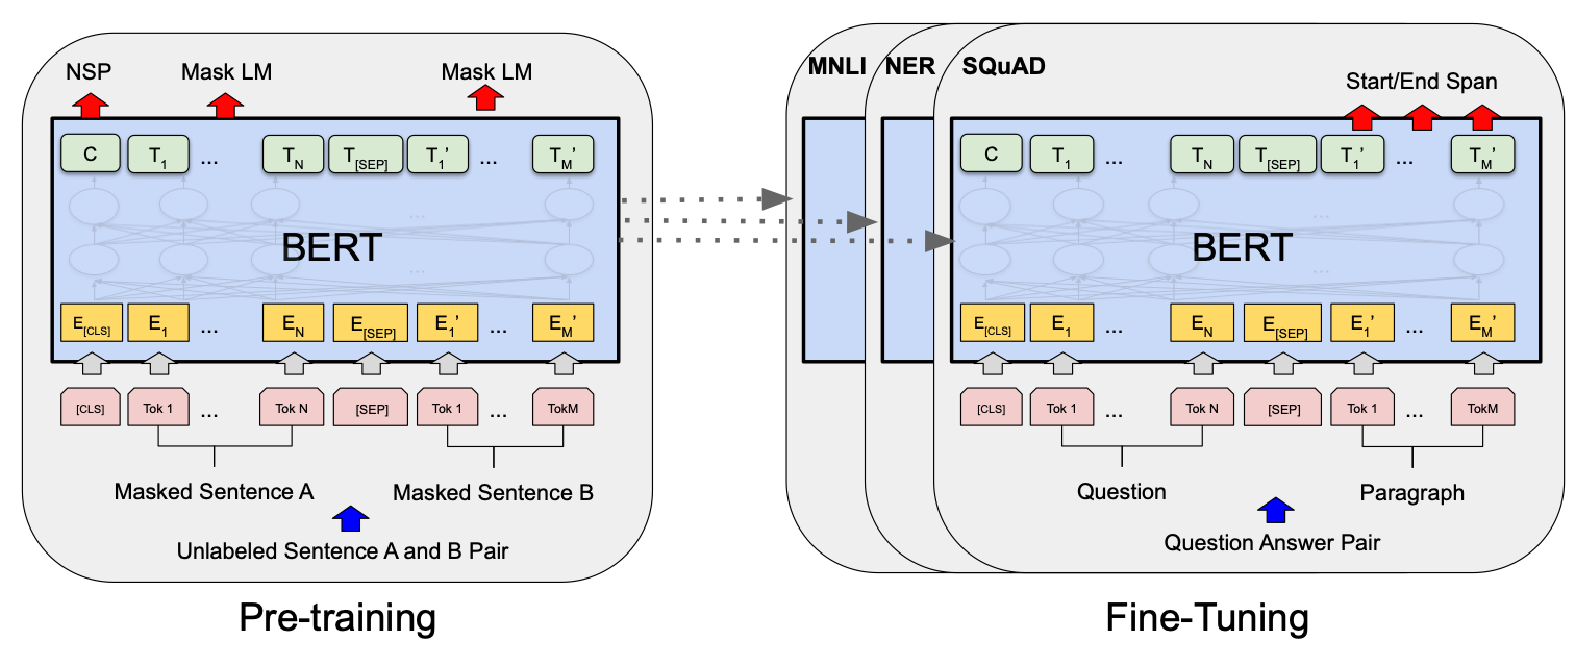
\includegraphics[width=.9\linewidth]{bert_aclanth_N19-1423_fig-1.pdf}
    \\{\tiny \cite[Figure 1]{devlin-etal-2019-bert}}
    \caption{\footnotesize Caption. Describe notations enough. Use the same symbols (as much as the same fonts) with the body text. Do not use invisible tiny fonts.\bf When you cite a figure or table from a paper, credit the paper explicitly.}
    \label{fig:architecture}
\end{figure}

\subsection{Table example/表の例}

\begin{table}[H] % forcing `here'
    \centering
    \scriptsize
    %\resizebox{\textwidth}{!}{% use if the table is too big to fit
    \begin{tabularx}{\linewidth}{r|p{3cm}L}
    \toprule
      Type of Presentation & Main Purpose & Point \\
    \midrule
      Academic Oral & 
       Conveying outcomes to wider audience& 
       Present minimally so that
       people understand your contributions.
       Do not show all results.
       Observe the assigned time limit.
       No need to make the material understandable without the presenter's explanation. 
       \\
       \\
      Academic Poster & 
       Discussion with focused people & 
       Present minimally so that
       people understand your contributions.
       Do not show all results.
       Do not write text; Make it visually understandable by viewing it, not by reading it. 
       Make your poster roughly understandable without the presenter's explanation. 
       \\
       \\
      Lab Seminar &
       Sharing the status, confirming its validity, and brushing up &
       Make the material concise but sufficient so that a knowledgeable person can reproduce your work.
       It must be mostly understandable without the presenter's explanation. 
       Skip detail to present orally in a reasonable time frame.
       \\
    \bottomrule
    \end{tabularx}
    %}%\resizebox
    \caption{\footnotesize Caption. Provide enough information so that the reader can understand the meanings of symbols and notations in the table}
    \label{tab:type_of_presentations}
\end{table}

\I When you show your results as a table, you must describe the meanings of the results (your interpretation) in text. Do not let the table be alone

\I Before showing the result table, you also need to explain what you did, why you did it, and how you did it.


\section{Plan/今後の計画}

\I List up anything you need to do but put priorities and due dates

\I A Gantt chart is a good way to show yearly schedule


\footnotesize
\bibliographystyle{apalike}
\bibliography{sample} % should be the same or include the bib file for \bibinput

\end{document}
